\begin{center}
\begin{figure}[h]
	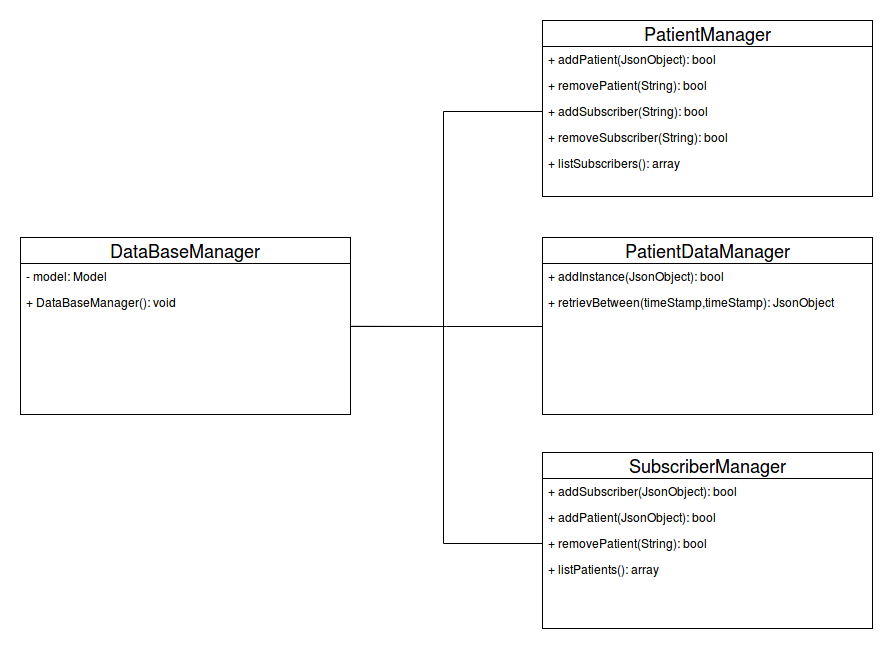
\includegraphics[width=15cm, height=13cm]{DataStorage/DataStorage.png}
\end{figure}
\end{center}

Follows is the description of each manager and the layout of the table that they will manage. It also discusses some of the specialized functions that they will provide.\\
\begin{itemize}
	\item DatabaseManager:\\
This is the parent class and it established the connection with the database. In the case that the database does not exit it will create one. It will do the same for all the tables specified to be in the database.\\

	\item PatientManager:\\
	This manager will store the identification of the patients on the system. Each patient will be able to obtain a list of all the individuals subscribed to their data, they will also have the ability to remove unwanted subscribers.\\


	\emph{Patient Table:}\\\\
		(Email, Password, Address, SubscriberPassword, PK(Username), Age, Weight, Height, Reason, SubscriberList)

\begin{itemize}
	\item Age: will be an Integer.
	\item Weight: will be a Double and will be measured in kilograms.
	\item Height: will be a Double and will be measured in metres.
	\item SubscriberList: will be a set of unique subscriber emails.
\end{itemize}
		
\item SubscriberManager:\\
This manager will store all the subscribers or general users. They will be identified by their email address. They will also have the ability to subscribe to patients, in which case the relevant information will be added to both the subscriber's list of patients and the patient's list of subscribers.\\

	\emph{Subscriber Table:}\\\\
		( PK(Email), Password, Relation, PatientList)\\
\begin{itemize}
		\item PatientList: will be a set of unique patient usernames.	\\
\end{itemize}

\item PatientDataManager:\\
This manager will have the functionality to retrieve patient data within a time span. The retrieveBetween function will preform this functionality and return a set containing an array of the patient data as well as the max, min and average value obtained during that time span.\\


	\emph{PatientData Table:}\\\\
		(PK(PatientUsername), PK(DeviceID), PK(TimeStamp), Value)\\
		\begin{itemize}
			\item Value: can be a double or a set of information.\\
		\end{itemize}
\end{itemize}		
	

Singleton pattern restricts the instantiation of a class and ensures that only one instance of the class exists in the java virtual machine. This is imperative for the databaseManager since we only to link with the database once regardless of the number of uses.

		
		